% !TEX root = ThesisGchatzi.tex

\chapter{Introduction} \label{chap:intro}

\section{Concept and Motivation}
\label{subsec:conept_motivation}

\textit{Time series} data is a treasure trove for a variety of mining and monitoring applications both in industry and in academia, while a rapidly increasing bulk of such data is also generated on the Web and the Internet of Things. They can represent various types of measurements, such as user check-ins at various Points of Interest (PoIs), energy consumption in smart buildings, PM2.5 particle concentration measured by air pollution sensors, etc. More formally, a time series is a time-ordered sequence of values. A real-world example of two time series representing the total per-hour water consumption during a specific day of two separate regions within a city, is illustrated in Figure~\ref{fig:ts_example}. Tasks such as exploring and mining time series data are highly important for discovering trends or patterns and extracting useful insights from such phenomena, having attracted extensive research interest over the last years \cite{DBLP:journals/pvldb/EchihabiZPB18,DBLP:conf/sigmod/LinardiZPK18a,DBLP:journals/datamine/YehZUBDDZSMK18,camerra2014kais,ding2008pvldb,shieh2008kdd}.

\begin{figure}[tb]
 \centering
 \includegraphics[width=0.5\textwidth]{water_ts.png}
\caption{Water consumption-related time series.}
\label{fig:ts_example}
\end{figure}

As an example of time series exploration, consider a large set of daily water consumption time series of a region within a city measured per hour, as the ones depicted in Figure~\ref{fig:ts_example}. Given a new time series, one could require to obtain the most similar one from the dataset, to detect days of similar consumption. However, looping over all time series in the dataset and comparing similarities could be rather time consuming. To speed things up, we could build an \textit{index} using all the time series in the dataset and then perform a similarity query on it. Several approaches have been proposed for efficiently indexing large amounts of time series data. One well-studied family of approaches includes wavelet-based methods \cite{chan1999icde}, which rely on \textit{Discrete Wavelet Transform} \cite{graps1995cse} to reduce the dimensionality of time series and generate an index using the coefficients of the transformed sequences. Another line of work employs a \textit{Symbolic Aggregate Approximation} (SAX) representation of time series \cite{jessica2007dmkd}, introducing a series of indices, such as $i$SAX~\cite{shieh2008kdd}, $i$SAX 2.0~\cite{camerra2010icdm}, $i$SAX2+~\cite{camerra2014kais}, and ADS+~\cite{zoumpatianos2014sigmod}.

However, to the best of our knowledge, none of the existing works so far has considered the specific case of \textit{geolocated time series} (i.e., produced at, or otherwise associated with, specific locations). Formally, geolocated time series can be defined as follows.

\begin{mydefinition} [Geolocated Time Series]
A {\em time series} is a time-ordered sequence of values $T = \{v_1, \ldots, v_w\}$, where $v_i$ is the value at the $i$-th time point and $w$ is the length of the series. A time series is \textit{geolocated} if it is also characterized by a location, denoted by $T.loc$. Assuming a 2-dimensional space, $T.loc_x$, $T.loc_y$ refer to the $(x,y)$ coordinates of $T$'s location.
\end{mydefinition}

Figure~\ref{subfig:geoTS} depicts a set of geolocated time series on a map. Geolocated time series can be found in various domains and applications. For instance, they can be used to represent, analyze and forecast water consumption measured by smart meters installed in urban households \cite{DBLP:conf/edbt/ChronisGA16}. Analyzing such time series can provide valuable insights regarding trends and patterns of consumer behavior in daily life. These results can then be used for customer segmentation, targeted marketing, planning future network upgrades, forecasting and balancing water demand, as well as planning and prioritizing interventions that can guide consumers towards more sensible water use. Similarly, check-ins in geosocial networks can also be modeled as geolocated time series. Analysis results can indicate nearby venues with similar frequency patterns, which may be used for social recommendations according to time, place, activity, etc. Other use cases can be found in other domains, such as in geomarketing or mobile advertisement, where geolocated time series may represent the number of visitors or the revenue generated at a certain location across time.

\begin{figure}[!tb]
 \centering
 \subfloat[Geolocated time series.]{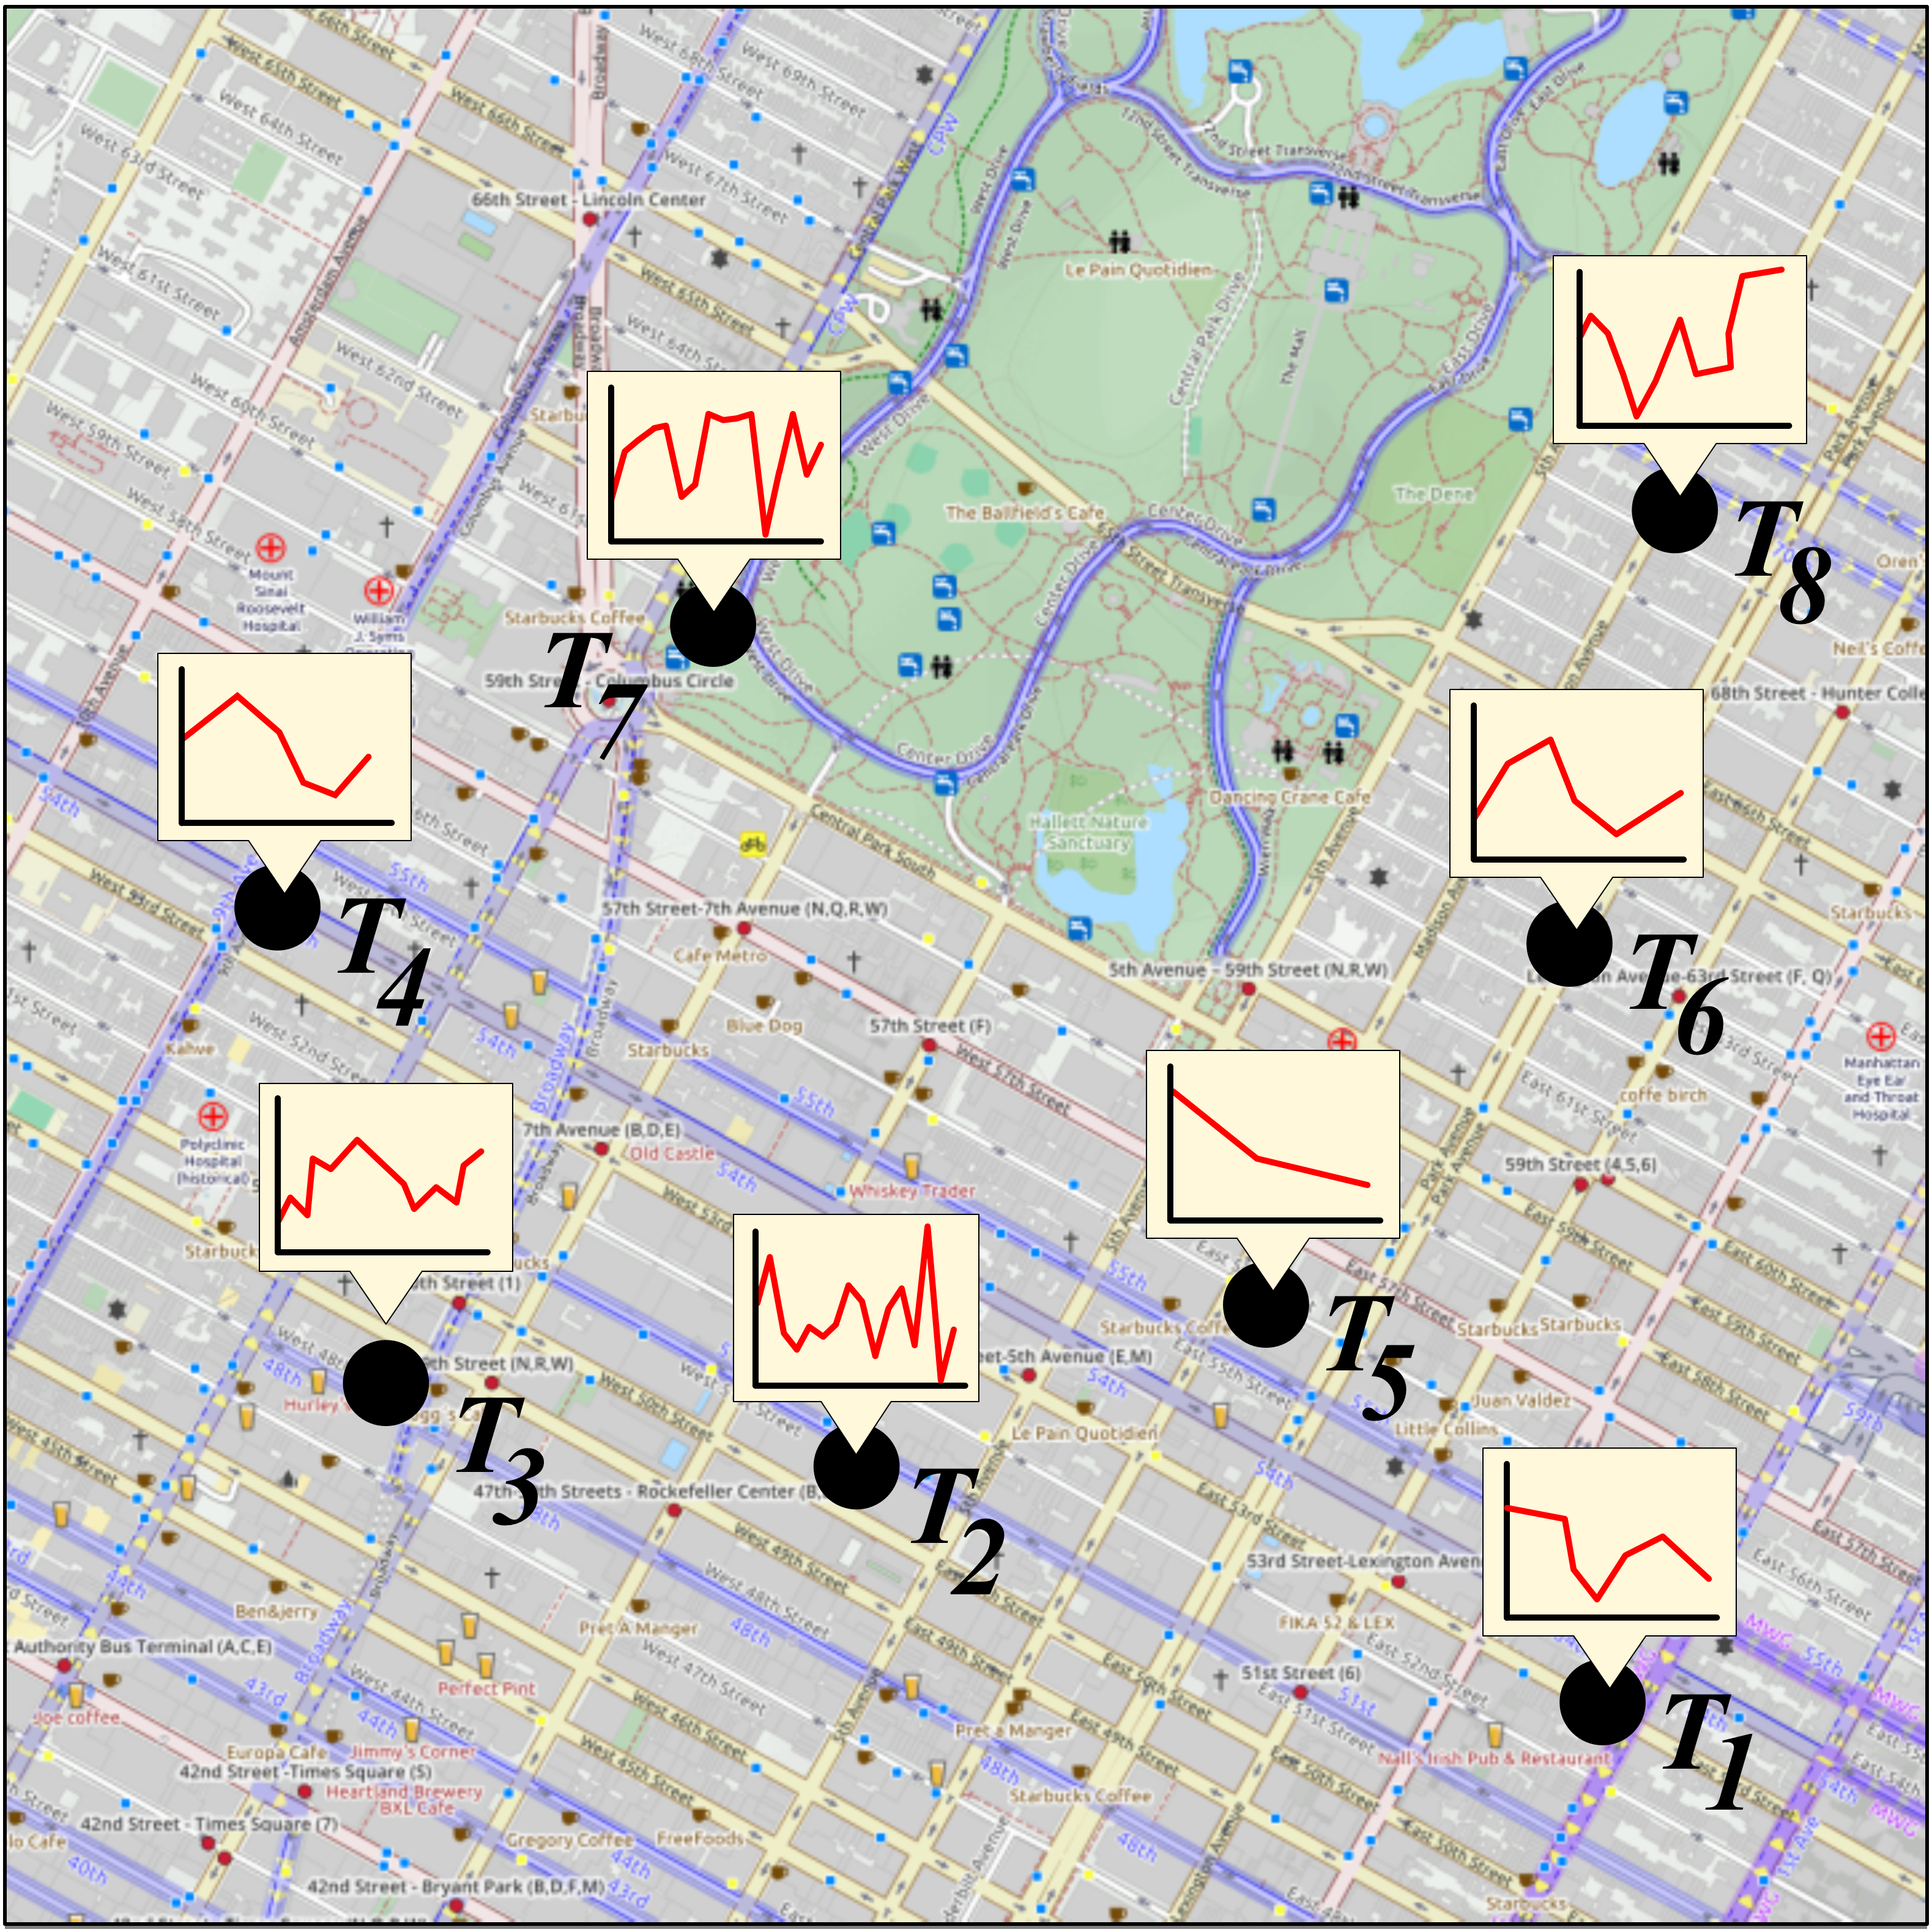
\includegraphics[width=0.4\textwidth]{geoTS.png}\label{subfig:geoTS}} \quad
 \subfloat[A query on geolocated time series.]{\includegraphics[width=0.4\textwidth]{geoTS_query.png}\label{subfig:geoTS_query}}
\caption{Examples of geolocated time series.}
\label{fig:geoTS_examples}
\end{figure}

All aforementioned indices aim at efficiently supporting \textit{similarity search} on time series data, based on similarity measures such as the \textit{Euclidean distance} and \textit{Dynamic Time Warping} (DTW); in case that the analyzed time series are associated with a spatial attribute and issued queries involve spatial filters, these need to be treated independently. As an example, given the set shown in Figure~\ref{subfig:geoTS} and a query geolocated time series, one could request all similar ones in the time domain that are also spatially close within a given range, as illustrated in Figure~\ref{subfig:geoTS_query} (i.e., the query geolocated time series is shaded green, while the results are blue). Thus, for such \textit{hybrid} queries employing both types of predicates, this implies evaluating each predicate separately. Other examples of hybrid queries involve retrieving the top-$k$ spatially closest geolocated time series that are also similar in the time series domain, or vice versa (i.e., top-$k$ most similar within a given range). Finally, a special type of such a query is the \textit{hybrid similarity join}, where, given two sets of geolocated time series, one could seek to retrieve \textit{all} possible spatially close pairs that are also similar in the time series domain. Of course, in all the above cases, due to the rather complex nature of time series data and in conjunction with the extra spatial characteristics, such analysis tasks can be a rather slow and cumbersome procedure, as the datasets get larger.

As mentioned, most research efforts on time series focus on similarity measures such as the Euclidean distance and dynamic time warping. These are globally calculated, i.e., across the entire length of time series. In this thesis, we introduce the measure of \textit{local similarity}, where we consider as similar, time series whose values do not differ by more than $\epsilon$ for at least $\delta$ consecutive timestamps. Based on this local similarity, and given a set of \textit{co-evolving} (i.e., time aligned) time series, we tackle the problem of detecting pairs and groups, called \textit{bundles}. These are pairs or groups of locally similar subsequences that could indicate common local patterns and trends. Hybrid \textit{local} similarity search on geolocated time series data is also of particular interest. For example, considering Figure~\ref{subfig:geoTS_query}, one could request all \textit{locally} similar time series within that area.

Extracting insights, trends and patterns from large geolocated time series datasets can be significantly facilitated by \textit{map-based visualizations} of \textit{summarized} time series data. For instance, considering the scenario of water consumption measured by smart meters installed in urban households, such visualizations could reveal which type of consumption patterns are most frequently observed among consumers in a certain area, or what the spatial distribution of sales for a certain product looks like. However, the inherently complex nature of time series, combined with the extremely large volumes of such datasets (i.e., millions or billions of geolocated time series), incommodes their management, analysis and exploration. In particular, visual exploration of geolocated time series needs to process the required information efficiently, while the user interacts with the application. For example, whenever the user zooms in or scrolls the map, visual analytics and aggregates should be computed on-the-fly, identifying the predominant patterns in the time series and their spatial distribution within the actual map area.

\textit{Forecasting} time series is crucially useful in various applications, such as resource demand management (e.g., water, electricity, natural gas), stock market and supply demand forecasting (e.g., in super markets). Applying forecasting \textit{simultaneously} on sets of time series can be a crucially useful task in such applications, where multiple forecasts should be available as soon as possible. Depending on the dataset (e.g., size, time series value heterogeneity), this can be a rather complex and computationally intensive task, due to the high dimensionality and usual uncertainty in such data. In this thesis, we focus on \textit{large scale}, simultaneous, distributed time series forecasting, that enables such analysis tasks on very large sets of time series (i.e., tens of millions).

\section{Contributions}
\label{subsec:contrib}

In the following, we provide details regarding all the contributions of this thesis on the above challenges.

\paragraph{Hybrid Indexing and Querying on Geolocated Time Series.} As mentioned, due to the rather complex nature of time series data, in conjunction with the extra spatial characteristics, executing hybrid similarity search queries can be a rather slow and cumbersome procedure. To make such applications more efficient and scalable, geolocated time series need to be appropriately \textit{indexed} to allow such queries based on both \textit{spatial proximity} and \textit{time series similarity}, enhancing the pruning potential. in this thesis, we introduce a \textit{hybrid index} for efficiently supporting similarity search on geolocated time series combining both \textit{spatial proximity} and \textit{time series similarity}. The proposed index, called \textit{\tsr}, extends the standard \textit{R-tree} by introducing \textit{bounds} for the time series indexed at each node. These bounds follow a similar intuition to the \textit{Minimum Bounding Rectangles} (MBR) of the R-tree, enclosing all the time series contained within a node. This reduces node accesses during query evaluation by simultaneously pruning the search space in the spatial domain and the time series domain. We also present an optimized version, the \textit{\btsr}, which uses tighter bounds by bundling together similar time series in each node. We describe how these indices can be used to efficiently evaluate different variants of hybrid queries combining spatial and time series filtering or ranking.

In the same line of work, we introduce efficient methods for applying \textit{hybrid similarity join} on very large geolocated time series datasets. A hybrid similarity join query aims to identify \textit{all pairs} between the two datasets qualifying to the criteria of spatial proximity and time series similarity. Clearly, performing a pairwise comparison among all pairs of objects in the two datasets is not an option when their size is large (i.e., millions of time series, each with several thousand data points or more). Hence, indexing them is indispensable for efficient processing of such queries. In this work, we take advantage of the \btsr's hybrid pruning potential, to deliver a more efficient and faster hybrid similarity join evaluation compared to other, adapted, state-of-the-art indices. However, this {\em centralized} approach has certain limitations, as it cannot sustain examination of large datasets. Hence, we further suggest a space-driven data partitioning scheme that enables a \textit{parallel and distributed} approach for hybrid similarity joins.

In summary, in the fields of hybrid indexing and querying on geolocated time series, our work makes the following contributions:

\begin{itemize}
 \item We propose the \tsr, a hybrid index for geolocated time series, extending the spatial R-tree and augmenting each node with appropriate time series bounds.
 \item We further optimize the \tsr to derive a more efficient variant, the BTSR-tree, that clusters the time series of each subtree to derive and maintain tighter bounds for pruning.
 \item We address the problem of similarity search for geolocated time series, via hybrid boolean or top-$k$ queries combining both spatial proximity and time series similarity.
 \item We adapt state-of-the-art indices (including the \btsr index) for hybrid similarity join over geolocated time series data in centralized settings and propose traversal methods that can prune the search space and return answers without false misses.
 \item We suggest a space-driven partitioning method to distribute large datasets in cluster infrastructures, thus enabling faster, in-parallel evaluation of smaller similarity join tasks.
 \item We experimentally validate our proposed approach using real-world datasets from different application use cases, showing that our hybrid indices can effectively allow simultaneous pruning of the search space in both spatial and time series domains, significantly reducing the required number of node accesses and execution time.
\end{itemize}

The above results are published at the International Conference on Advances in Geographic Information Systems (SIGSPATIAL) 2017~\cite{chatzig17btsr} and 2018~\cite{chatzigeorgakidis2018scalable}.

%%%%%%%% VISUALIZATION
\paragraph{Visual Exploration of Geolocated Time Series.} In this thesis, we propose two geolocated time series \textit{summarization} approaches for visual exploration. These are supported and driven by two hybrid indices (i.e., an adapted variant of \btsr and a hybrid variant of \isax index, called \textit{\hisax}) that speed up the result computation, providing efficient exploration of geolocated time series data. They consist of a spatial and a time series summary that jointly facilitate knowledge extraction and insight gaining. To the best of our knowledge, this is the first work that considers visual exploration and summarization of geolocated time series. In brief, our main contributions on this field are the following:

\begin{itemize}
 \item We suggest an adapted variant of the \btsr index, as well as a novel algorithm for its traversal in order to quickly retrieve summaries of geolocated time series within a given spatial area.
 \item We propose a hybrid variant of the \isax index, called \hisax, which combines time series with spatial information within its nodes. Based on that, we describe a novel traversal algorithm for \hisax that enables fast \textit{timebox} (i.e., a rectangle in the time series domain) search by performing efficient pruning, while avoiding false negatives.
 \item We exemplify the proposed visualization methods with two use cases based on real-world datasets. In addition, we empirically evaluate the performance of our summarization methods, confirming their low execution time against a large synthetic dataset of geolocated time series.
\end{itemize}

A preliminary version of the above results appears at the BigVis workshop, which was held in conjunction with EDBT/ICDT 2018 joint conference~\cite{chatzigeorgakidis2018map}. The complete work is published at the Elsevier Big Data Research journal~\cite{chatzigeorgakidis2019visual} in 2019.

%%%%%%%% LOCAL SIMILARITY
\paragraph{Local Similarity Search.} Towards the efficient detection of pairs and bundles of locally similar co-evolving time series, we first present a baseline algorithm that performs a sweep line scan across all timestamps to identify matches. Then, we propose a filter-verification technique that only examines candidate matches at judiciously chosen checkpoints across time. Specifically, we introduce two block scanning algorithms for discovering local pairs and bundles respectively, which leverage the potential of checkpoints to aggressively prune the search space.

In the same line of work, we tackle the problem of similarity search on geolocated time series data, using local similarity. Our approach for hybrid search over geolocated time series using the \btsr supports only \textit{global} geolocated time series similarity. Such hybrid queries involving local similarity can also be evaluated using the \btsr index. We first present a baseline method employing a sweep-line algorithm to check for local similarity, and then describe how this can be optimized by using appropriately placed checkpoints, based on the local similarity score threshold specified by the query, in order to skip unnecessary comparisons. Despite the fact that this saves some computations, the resulting time savings are relatively small, since the number of index nodes that need to be probed is not significantly reduced. To overcome this problem, we introduce an improvement to the \btsr index, which is based on temporally \textit{segmenting} the time series bounds within each node and deriving tighter bounds per segment. Once the time series bounds in each node become more fine-grained, pruning the search space for local similarity queries proves much more effective.

%Contribution
Our main contributions on pair/bundle discovery and local similarity search can be summarized as follows:

\begin{itemize} 
 \item We introduce the problems of local pair and bundle discovery over co-evolving time series.
 \item We suggest an aggressive checkpoint-based pruning method that drastically reduces the candidate pairs and bundles that need to be verified, significantly improving performance.
 \item We conduct an extensive experimental evaluation using both real-world and synthetic time series, showing that our algorithms outperform the respective sweep line baselines.
 \item We extend our previous work on hybrid queries for geolocated time series to support local time series similarity. We consider both range and top-$k$ queries, including combined criteria for spatial distance and local time series distance.
 \item We present how such queries can be answered efficiently exploiting the \btsr index.
 \item To achieve lower execution time by further reducing node accesses, we propose an enhanced variant of \btsr, called \sbtsr, which additionally employs temporal segmentation in each node to derive tighter, more fine-grained time series bounds.
 \item We experimentally evaluate our methods using real-world datasets from different application domains, showing that \btsr can efficiently handle hybrid queries under local similarity search, while \sbtsr achieves even higher performance due to the additional temporal segmentation.
\end{itemize}

The above results are published at the 16th International Symposium on Spatial and Temporal Databases (SSTD) 2019~\cite{chatzigeorgakidis2019local} and at the International Conference on Advances in Geographic Information Systems (SIGSPATIAL) 2019~\cite{chatzigeorgakidis2019geolocal}.

\paragraph{Scalable Time Series Forecasting.} To support large scale, simultaneous time series forecasting, we introduce a framework for scalable data analysis on Big Data collections, named \textit{FML-$k$NN} (i.e., Flink Machine Learning $k$-Nearest Neighbors). The framework implements a probabilistic classifier and a regressor. Its core algorithm is an extension of \textit{F-$zk$NN}~\cite{chatzigeorgakidis2015mapreduce}, which is built upon an optimized version of the \textit{H-$zk$NNJ}~\cite{zhang2012epk} distributed approximate $k$NN join algorithm. Finally, we demonstrate the framework's capabilities through a large scale time series forecasting use-case on a large real-world dataset of hourly water consumption per household within a city.

The overall contributions of our work on FML-$k$NN are the following:
\begin{itemize}
	\item We propose a novel, easily extensible distributed processing framework that performs probabilistic classification and regression using $k$NN join.
	\item The framework operates in a single distributed session, saving I/O and communication resources. Similar approaches require three distributed sessions.
	\item We present a detailed experimental and comparative evaluation with similar approaches and exhibit our framework's efficiency in terms of scalability and wall-clock completion time.
	\item We conduct experiments on two real-world cases using water consumption related datasets and extract useful knowledge and insights towards the induction of more efficient water use.
\end{itemize}

A preliminary version of these results appears at the 2015 IEEE International Conference on Big Data (BigData)~\cite{chatzigeorgakidis2015mapreduce}. The complete work is published at the Springer Journal of Big Data~\cite{chatzigeorgakidis2018fml} in 2018.

\section{Organization}
\label{sec:org}

The rest of this thesis is structured as follows:

\begin{description}
	\item Chapter~\ref{chap:related} surveys the related work in the field of time series indexing, querying, exploration and similarity search, as well as scalable $k$NN methods and machine learning.
	\item Chapter~\ref{chap:btsr} presents our hybrid \btsr index, that indexes geolocated time series both in the spatial and in the time series domain.
	\item Chapter~\ref{chap:btsr_queries} extends the work of Chapter~\ref{chap:btsr}, introducing a variety of hybrid queries that can be processed using the \btsr index.
	\item Chapter~\ref{chap:vis} considers an efficient exploration on large geolocated time series data, using hybrid indexing.
	\item Chapter~\ref{chap:local_sim} introduces the pair and bundle discovery on large co-evolving time series datasets based on local similarity. It also presents a new collection of hybrid local similarity search queries, using hybrid indexing.
	\item Chapter~\ref{chap:knn} considers scalable $k$NN joins and presents our FML-$k$NN framework for classification and regression on Big Data.
	\item Chapter~\ref{chap:conclusions} concludes this thesis and presents future work directions.
\end{description}